\documentclass{standalone}
\usepackage{tikz}

\usetikzlibrary{positioning}

\begin{document}
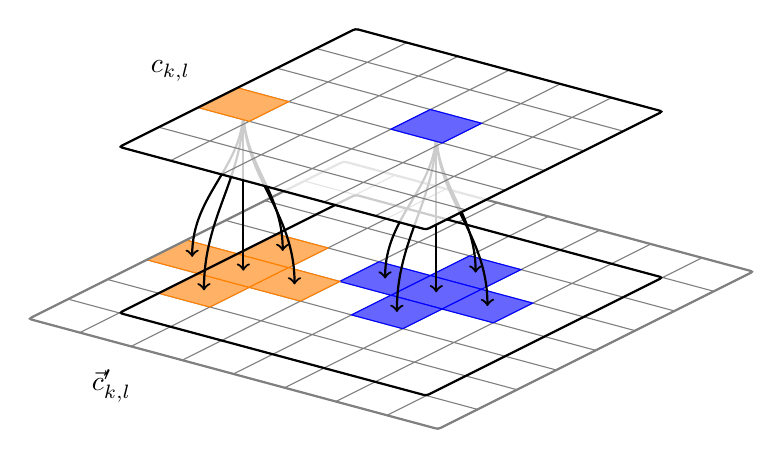
\begin{tikzpicture}[scale=1,every node/.style={minimum size=0.5cm},on grid]

  \begin{scope}[
      yshift=-100,
      every node/.append style={yslant=0.5, xslant=-1.3},
      yslant=0.5,
      xslant=-1.3
    ]
    \coordinate (c32) at (1.75, 1.25);
    \coordinate (co25) at (1.25, 2.75);
  \end{scope}

  \begin{scope}[
      yshift=-160,
      every node/.append style={yslant=0.5, xslant=-1.3},
      yslant=0.5,
      xslant=-1.3
    ]
    \coordinate (cp42) at (2.25, 1.25);
    \coordinate (cp32) at (1.75, 1.25);
    \coordinate (cp22) at (1.25, 1.25);
    \coordinate (cp33) at (1.75, 1.75);
    \coordinate (cp31) at (1.75, 0.75);

    \coordinate (cop15) at (0.75, 2.75);
    \coordinate (cop25) at (1.25, 2.75);
    \coordinate (cop35) at (1.75, 2.75);
    \coordinate (cop24) at (1.25, 2.25);
    \coordinate (cop26) at (1.25, 3.25);
  \end{scope}

  % lower plane
  \begin{scope}[
      yshift=-160,
      every node/.append style={yslant=0.5, xslant=-1.3},
      yslant=0.5,
      xslant=-1.3
    ]
    \draw[step=5mm, thin, gray] (-0.5,-0.5) grid (3.5,3.5);

    \fill[blue!60] (2,1) rectangle (2.5,1.5);
    \node at (cp42) [draw, color=blue] {};%{$c^\prime_{4,2}$};

    \fill[blue!60] (1.5,1) rectangle (2.0,1.5);
    \node at (cp32) [draw, color=blue] {};%{$c^\prime_{3,2}$};

    \fill[blue!60] (1,1) rectangle (1.5,1.5);
    \node at (cp22) [draw, color=blue] {};%{$c^\prime_{2,2}$};

    \fill[blue!60] (1.5,1.5) rectangle (2.0,2.0);
    \node at (cp33) [draw, color=blue] {};%{$c^\prime_{3,3}$};

    \fill[blue!60] (1.5,0.5) rectangle (2.0,1.0);
    \node at (cp31) [draw, color=blue] {};%{$c^\prime_{3,1}$};

    \fill[orange!60] (0.5,2.5) rectangle (1.0,3.0);
    \node at (cop15) [draw, color=orange] {};%{$c^\prime_{1,5}$};

    \fill[orange!60] (1.0,2.5) rectangle (1.5,3.0);
    \node at (cop25) [draw, color=orange] {};%{$c^\prime_{2,5}$};

    \fill[orange!60] (1.5,2.5) rectangle (2.0,3.0);
    \node at (cop35) [draw, color=orange] {};%{$c^\prime_{3,5}$};

    \fill[orange!60] (1.0,2.0) rectangle (1.5,2.5);
    \node at (cop24) [draw, color=orange] {};%{$c^\prime_{2,4}$};

    \fill[orange!60] (1.0,3.0) rectangle (1.5,3.5);
    \node at (cop26) [draw, color=orange] {};%{$c^\prime_{2,6}$};

    \draw[black,thick, rounded corners=1] (0,0) rectangle (3,3);
    \draw[gray,thick, rounded corners=1] (-0.5,-0.5) rectangle (3.5,3.5);
  \end{scope}

  % arrows
  \begin{scope}
    \draw[>->, thick] (c32) node[left,scale=1.3] {} to[out=270,in=90] (cp42);
    \draw[>->, thick] (c32) node[left,scale=1.3] {} to[out=270,in=90] (cp32);
    \draw[>->, thick] (c32) node[left,scale=1.3] {} to[out=270,in=90] (cp22);
    \draw[>->, thick] (c32) node[left,scale=1.3] {} to[out=270,in=90] (cp33);
    \draw[>->, thick] (c32) node[left,scale=1.3] {} to[out=270,in=90] (cp31);

    \draw[>->, thick] (co25) node[left,scale=1.3] {} to[out=270,in=90] (cop24);
    \draw[>->, thick] (co25) node[left,scale=1.3] {} to[out=270,in=90] (cop25);
    \draw[>->, thick] (co25) node[left,scale=1.3] {} to[out=270,in=90] (cop26);
    \draw[>->, thick] (co25) node[left,scale=1.3] {} to[out=270,in=90] (cop15);
    \draw[>->, thick] (co25) node[left,scale=1.3] {} to[out=270,in=90] (cop35);
  \end{scope}

  % upper plane
  \begin{scope}[
      yshift=-100,
      every node/.append style={yslant=0.5, xslant=-1.3},
      yslant=0.5,
      xslant=-1.3
    ]
    \fill[white,fill opacity=0.8] (0,0) rectangle (3,3);
    \draw[step=5mm, thin, gray] (0,0) grid (3,3);

    \fill[blue!60] (1.5,1) rectangle (2.0,1.5);
    \node at (c32) [draw, color=blue] {};%{$c_{3,2}$};

    \fill[orange!60] (1.0,2.5) rectangle (1.5,3.0);
    \node at (co25) [draw, color=orange] {};%{$c_{2,5}$};

    \draw[black,thick, rounded corners=1] (0,0) rectangle (3,3);
  \end{scope}

  \node at (-3.25cm,-1.5cm) [black] {$c_{k,l}$};
  \node at (-4cm,-5.5cm) [black] {$\vec{c}^\prime_{k,l}$};
\end{tikzpicture}
\end{document}
